%====================================================================================
\section{Ruido Blnaco}
%====================================================================================

\begin{frame}{Procesos estocásticos elementales: Ruido Blanco}
	El denominado \textit{ruido blanco} es un proceso estocástico que presenta media nula, varianza constante y sin correlación con su pasado, si además la distribución es normal, se denomina \textit{Ruido Blanco Gaussiano}.
	\begin{align*}
		E(a_t) & = 0\\
		E(a_t^2) & = \sigma_{a}^2\\
		Cov(a_t, a_{t+k}) & = 0 \quad \forall k
	\end{align*}
	La función de autocovarianza y autocorrelación para este proceso sería:
	\begin{equation*}
		\gamma_k =	\begin{cases}
			\sigma^2&, k=0 \\
			0 &,  k \geq
		\end{cases} \qquad
		\widehat{\rho}_k =	\begin{cases}
			1 &, k= 0\\
			0 &, k \geq
		\end{cases}
	\end{equation*}
\end{frame}
%---------------------------------------------------
\begin{frame}{Correlograma de un ruido blanco}
	\centering
	\begin{figure}
		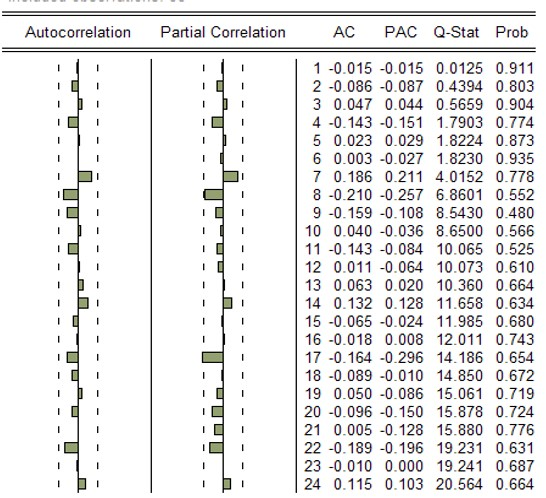
\includegraphics[width = 0.75\linewidth]{fig/figure6.jpg}
	\end{figure}
\end{frame}
%---------------------------------------------------
\begin{frame}{Procesos estocásticos elementales: Ruido Blanco}
	\begin{itemize}
		\item Con frecuencia interesa evaluar si una serie se aproxima razonablemente bien con un RB, lo cual equivale a averiguar si todas sus correlaciones son igual a cero.
		\item Un resultado fundamental es que en una serie que es RB, la distribución de autocorrelaciones muestrales con grandes muestras es:
			$$\rho_k \thicksim \mathcal{N}\left(0, \frac{1}{T} \right) $$
		\item Así, si la serie es RB, casi el 95\% de las autocorrelaciones muestrales deben caer en el intervalo $\pm 2/Raíz(T)$. Ver intervalos de confianza en los correlogramas.
	\end{itemize}
\end{frame}
%---------------------------------------------------
\begin{frame}{Procesos estocásticos elementales: Ruido Blanco}
	\begin{itemize}
		\item Un test que permite probar si todas las autocorrelaciones son 0 de manera conjunta, se deriva de la expresión:
			$$\rho_k \thicksim \mathcal{N}\left(0, \frac{1}{T} \right) \rightarrow \sqrt{T}\rho_k \thicksim \mathcal{N}(0,1) \rightarrow T\rho_k^2 \thicksim \chi_1^2$$
		\item Al recordar que la suma de variables independientes Chi-Cuadrado es también una chi con grados de libertad igual a la suma, hemos demostrado el \textcolor{red}{estadístico Q de Box-Pierce} cuya \textcolor{red}{hipótesis nula es que la serie es RB}
			$$\mathcal{Q}_{BP} = T\sum_{k=1}^{m}\rho_k^2$$
	\end{itemize}
\end{frame}
%---------------------------------------------------
\begin{frame}{Procesos estocásticos elementales: Ruido Blanco}
	\begin{itemize}
		\item  Una pequeña variación del test anterior apropiado para muestras pequeñas es el \textcolor{red}{test de Ljung-Box}:
			$$\mathcal{Q}_{BP} = T(T+2)\sum_{k=1}^{m}\left(\frac{1}{T-K} \right) \rho_k^2$$
		\item Siendo la diferencia que ahora las autocorrelaciones se encuentran ponderadas de tal forma que se le da más importancia a los rezagos lejanos.
	\end{itemize}
\end{frame}
%---------------------------------------------------
\begin{frame}{De nuevo el Correlograma de un RB}
	\centering
	\begin{figure}
		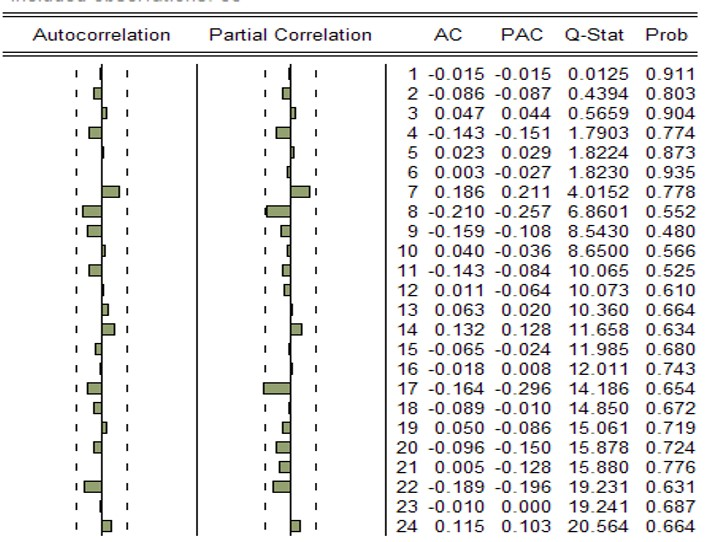
\includegraphics[width = 0.75\linewidth]{fig/figure7.jpg}
	\end{figure}
\end{frame}